\documentclass[11pt,a4paper]{article}
\usepackage[utf8]{inputenc}
\usepackage[T1]{fontenc}
\usepackage[brazil]{babel}
\usepackage[margin=2.4cm]{geometry}
\usepackage{booktabs}
\usepackage{amsmath,amssymb}
\usepackage{caption}
\usepackage{graphicx}
\usepackage{setspace}
\usepackage[hidelinks]{hyperref}
\graphicspath{{docs/}}
\onehalfspacing
\captionsetup{font=small,labelsep=colon}

\title{\textbf{Resultados II}\\[3pt]
\large O modelo de demanda com ajuste parcial da carteira:\\
formalização e estimação das anotações do orientador\\[4pt]
\normalsize Peso de VALE3 nos fundos do Itaú, 2016--2021}
\author{João Paulo Zangrandi \quad (orientador: Prof.\ Maurício Ferraresi Jr.)}
\date{\today}

\begin{document}
\maketitle

\begin{abstract}
\noindent Este documento formaliza, com equações, tabelas e interpretações, tudo o que consta nas
duas folhas manuscritas do orientador: o objeto e a especificação de demanda (peso desejado como
produto entre características do fundo e fatores latentes da ação), a estimação do fator por seção
transversal (linear e logística), a dinâmica de ajuste parcial da carteira, a estimação da
velocidade de ajuste por mínimos quadrados e por variável instrumental, o erro de previsão do peso,
a caracterização de sua série temporal e a regra de decisão sob a opacidade de 90 dias. Todos os
números vêm dos scripts em R do repositório (\texttt{R/24}--\texttt{R/30}).
\end{abstract}

\tableofcontents
\bigskip

% =====================================================================
\section{Objeto e especificação de demanda (folha 1)}

\paragraph{Objeto.} Consideram-se todos os fundos $i$ de uma gestora $M$ (o grupo Itaú) que detêm
uma ação $n$ (VALE3), no painel mensal 2016--2021 (72 meses). O alvo é o peso $w_{i,t}\in[0,1]$ da
ação em cada fundo.

\paragraph{Peso desejado + componente estocástico.} A cada mês, o peso observado é decomposto em um
peso desejado mais um erro,
\begin{equation}
w_{i,n} = w^{*}_{i,n} + \varepsilon_{i,n}, \qquad w^{*}_{i,n} = x_i'\,\theta_n,
\label{eq:demanda}
\end{equation}
em que $x_i$ é o vetor de $K$ \emph{características do fundo} (os \emph{investor embeddings} da folha:
tamanho, cotistas, tipo de fundo, fluxo) e $\theta_n$ é o vetor de $K$ \emph{fatores latentes da
ação} (os \emph{asset embeddings}: o quanto cada característica ``puxa'' a posição em VALE3). É a
versão em quantidades de um sistema de demanda à Koijen e Yogo (2019): fixa-se o ativo e faz-se o
peso depender do perfil do fundo.

\paragraph{Estimação do fator (seção transversal).} Empilhando os fundos vivos no mês $t$, com as
características em z-score, o vetor de fatores é estimado por mínimos quadrados,
\begin{equation}
w_n = X\,\theta_n + \varepsilon_n, \qquad
\widehat{\theta}_n = (X'X)^{-1} X'\,w_n .
\label{eq:ols_theta}
\end{equation}
Como anota a folha, as estimativas são, a rigor, \textbf{não lineares}, pois o peso é uma fração e a
forma correta usa uma ligação logística,
\begin{equation}
w_{i,n} = g\!\left(x_i'\theta_n\right) + \varepsilon_{i,n}, \qquad g(z)=\frac{1}{1+e^{-z}} .
\label{eq:logit}
\end{equation}

\subsection{Resultados do primeiro passo}

A Tabela~\ref{tab:theta} traz o fator $\widehat{\theta}_t$ resumido no estilo Fama--MacBeth (média
dos 72 meses, erros-padrão Newey-West). Os sinais são estáveis nos 72 meses: fundos maiores têm
menos VALE3 em peso; mais cotistas, mais peso; fundo de cotas, menos posição direta; o fluxo não
explica o nível.

\begin{table}[h]\centering\small
\caption{Fator latente $\widehat\theta_t$: regressão transversal do peso, padronizada (Fama--MacBeth,
72 meses; erros-padrão Newey-West).}
\label{tab:theta}
\begin{tabular}{@{}lrrrc@{}}
\toprule
Característica & Coeficiente & Erro padrão (NW) & Estatística $t$ & Significância \\
\midrule
Intercepto (nível médio)      & $0{,}03956$ & $0{,}00377$ & $10{,}5$  & *** \\
$\ln$(patrimônio) por d.p.    & $-0{,}00681$ & $0{,}00061$ & $-11{,}2$ & *** \\
$\ln$(cotistas) por d.p.      & $0{,}01087$  & $0{,}00099$ & $10{,}9$  & *** \\
Fundo de cotas                & $-0{,}01697$ & $0{,}00151$ & $-11{,}3$ & *** \\
Captação / patrimônio         & $-0{,}00044$ & $0{,}00412$ & $-0{,}1$  & não signif. \\
\bottomrule
\end{tabular}
\caption*{\footnotesize $R^2$ médio por mês $=0{,}152$. Três asteriscos: significância a um por mil.
Fonte: \texttt{R/24}.}
\end{table}

A versão logística confirma a leitura (Tabela~\ref{tab:logit}): mesmos sinais e significância, e o
efeito parcial médio (em pontos de peso por desvio-padrão) praticamente coincide com o linear. A
vantagem da logística é respeitar o suporte: o modelo linear prevê pesos fora de $[0,1]$ em
$2{,}51\%$ das observações, ao passo que a logística nunca (pseudo-$R^2$ de $0{,}165$ contra
$0{,}152$).

\begin{table}[h]\centering\small
\caption{Fator logístico (resposta fracionária), Fama--MacBeth com Newey-West.}
\label{tab:logit}
\begin{tabular}{@{}lrrrrc@{}}
\toprule
Característica & Coef.\ (chances log.) & Erro padrão (NW) & Est.\ $t$ & Efeito parcial (p.p.) & Sig. \\
\midrule
Intercepto            & $-3{,}380$ & $0{,}150$ & $-22{,}5$ & --- & *** \\
$\ln$(patrimônio)     & $-0{,}339$ & $0{,}043$ & $-7{,}9$  & $-0{,}68$ & *** \\
$\ln$(cotistas)       & $0{,}469$  & $0{,}035$ & $13{,}3$  & $+1{,}06$ & *** \\
Fundo de cotas        & $-0{,}732$ & $0{,}062$ & $-11{,}7$ & $-1{,}60$ & *** \\
Captação / patrimônio & $0{,}078$  & $0{,}183$ & $0{,}4$   & $\approx 0$ & não signif. \\
\bottomrule
\end{tabular}
\caption*{\footnotesize O efeito parcial médio é a resposta do peso em pontos percentuais por
desvio-padrão, comparável ao coeficiente linear. Fonte: \texttt{R/25}.}
\end{table}

\subsection{Dinâmica do fator}

Os coeficientes $\theta_t$ variam no tempo, mas revertem à média (Figura~\ref{fig:theta};
autocorrelação de $0{,}37$ a $0{,}84$, teste de Dickey--Fuller rejeitando raiz unitária em quatro
das cinco séries). Isso justifica tratá-los como um fator dinâmico e prever com passeio aleatório,
processo autorregressivo ou filtro de Kalman.

\begin{figure}[h]\centering
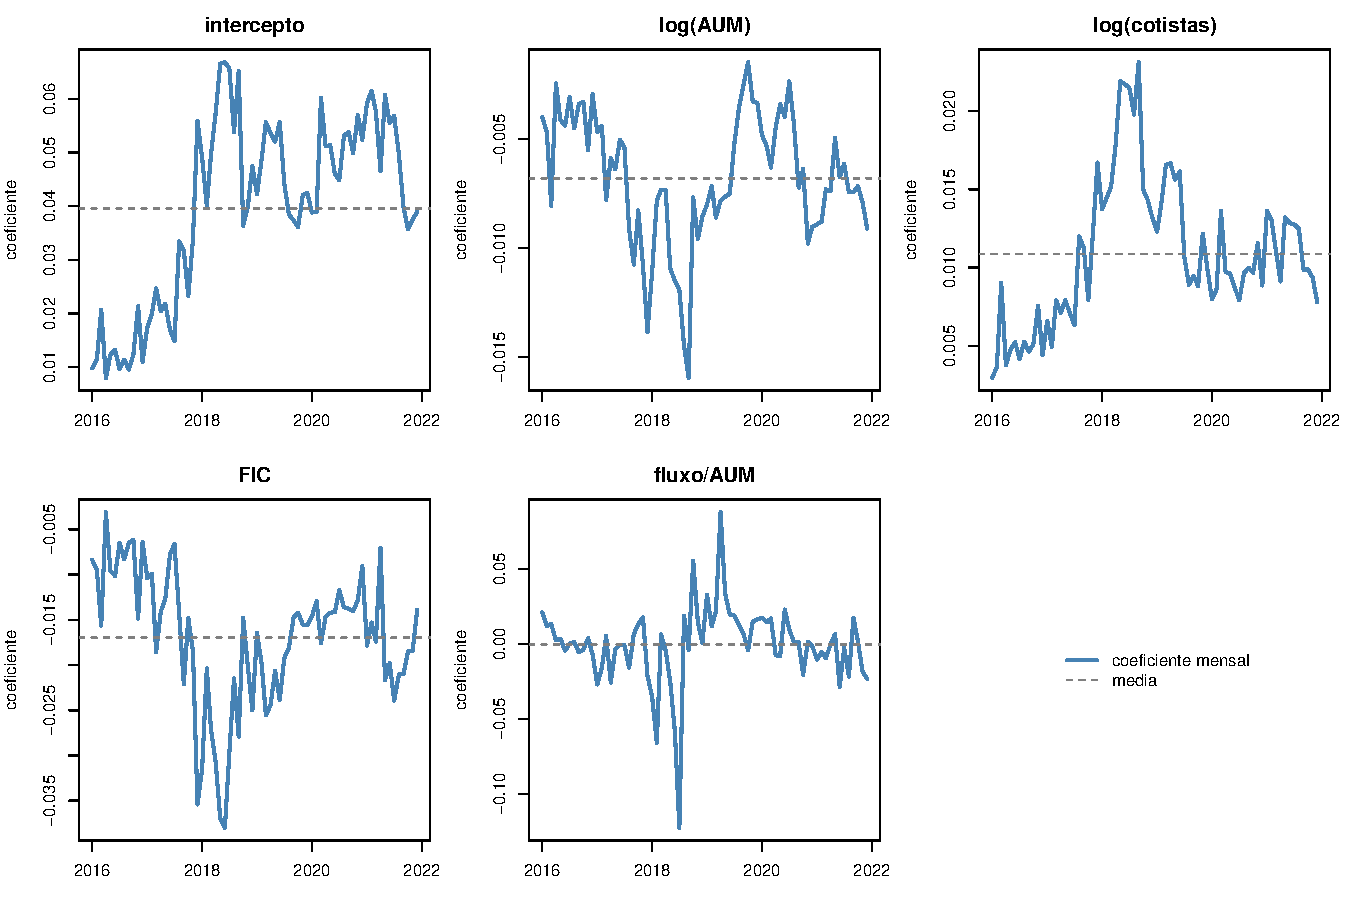
\includegraphics[width=0.80\textwidth]{fig_theta_padr.pdf}
\caption{Coeficientes padronizados $\widehat\theta_t$ da regressão mês a mês (2016--2021); tracejado
$=$ média. Fonte: \texttt{R/29}.}
\label{fig:theta}
\end{figure}

% =====================================================================
\section{Ajuste parcial da carteira (folha 1)}

A segunda parte da primeira folha liga um mês ao outro. A hipótese é que o fundo não salta para o
peso desejado de uma vez, mas se move parcialmente em sua direção, a uma velocidade $\lambda_n$:
\begin{equation}
w_{i,t+1} = (1-\lambda_n)\,w_{i,t} + \lambda_n\,w^{*}_{i,t} + u_{i,t+1}.
\label{eq:pa1}
\end{equation}
Reagrupando, a variação do peso é proporcional à distância que faltava para o alvo,
\begin{equation}
w_{i,t+1} - w_{i,t} = \lambda_n\,\big(\underbrace{w^{*}_{i,t}-w_{i,t}}_{\displaystyle \varepsilon_{i,t}\ \equiv\ d_{i,t}}\big) + u_{i,t+1},
\qquad\text{ou}\qquad
d_{n,t+1} = \lambda_n\,\varepsilon_{n,t} + u_{i,t+1}.
\label{eq:pa2}
\end{equation}
Aqui a folha usa $\varepsilon_{i,t}=w^{*}_{i,t}-w_{i,t}$ para a distância ao alvo e $d_{n,t+1}$ para a
variação do peso; para evitar confusão com o resíduo da seção transversal, chamamos a distância de
$d_{i,t}$. A constante $\lambda_n$ é a velocidade de ajuste: $\lambda=1$ ajusta tudo na hora,
$\lambda=0$ mantém o peso preso no valor de ontem.

% =====================================================================
\section{Estimação da velocidade $\lambda$ (folha 2, topo)}

\paragraph{O estimador de mínimos quadrados (a equação circulada no topo da folha 2).} A forma
direta é a de mínimos quadrados, escrita nas equações normais,
\begin{equation}
\widehat{\lambda}^{\,\text{MQO}}_n = \big(\widehat{\varepsilon}_{nt}'\,\widehat{\varepsilon}_{nt}\big)^{-1}
\widehat{\varepsilon}_{nt}'\,d_{n,t+1}
= \big(d_{n,t}'\,d_{n,t}\big)^{-1} d_{n,t}'\,(w_{n,t+1}-w_{n,t}).
\label{eq:lambdaols}
\end{equation}
Ao lado dela a folha anota ``provavelmente \emph{ridge} regression''. Essa intuição inicial,
contudo, foi revista: como a distância $d_{i,t}=g(x_{i,t}'\widehat{\theta}_t)-w_{i,t}$ é construída
com o fator \emph{estimado} $\widehat{\theta}_t$, ela é um regressor medido com erro. Sob erro nas
variáveis, o mínimos quadrados sofre \textbf{viés de atenuação} (puxa $\widehat\lambda$ para zero);
e, como o próprio $w_{i,t}$ aparece nos dois lados de \eqref{eq:pa2}, há ainda uma reversão à média
mecânica que puxa para cima. Uma regularização \emph{ridge} também encolhe para zero e, por isso,
\emph{agravaria} a atenuação --- justamente contra o teste de interesse (é $\lambda\neq0$?). O
\emph{ridge} fica, então, reservado a um passo futuro (estimar $\theta$ em dimensão alta), não a
este.

\paragraph{A correção por variável instrumental.} Usa-se como instrumento a distância defasada
$d_{i,t-1}$, em dois estágios. No primeiro, projeta-se a distância corrente sobre o instrumento,
$d_{i,t}=\pi\,d_{i,t-1}+v_{i,t}$, retendo a parte $\widehat{d}_{i,t}=\widehat\pi\,d_{i,t-1}$ ---
a componente previsível pelo mês anterior, limpa do ruído corrente. No segundo, regride-se a
variação do peso sobre essa parte limpa, o que, no caso exatamente identificado, dá
\begin{equation}
\widehat{\lambda}^{\,\text{VI}}_n =
\frac{\sum_{i,t} d_{i,t-1}\,(w_{i,t+1}-w_{i,t})}{\sum_{i,t} d_{i,t-1}\,d_{i,t}} .
\label{eq:lambdaiv}
\end{equation}
O instrumento é forte ($\widehat\pi\approx0{,}9$), correlacionado com a distância verdadeira mas não
com o ruído de medida, corrigindo os dois vieses de uma vez.

\subsection{Resultados de $\lambda$}

\begin{table}[h]\centering\small
\caption{Velocidade de ajuste $\lambda$ na equação $\Delta w_{i,t+1}=\lambda\,d_{i,t}+u$.
Erro-padrão agrupado por fundo ($10.570$ observações).}
\label{tab:lambda}
\begin{tabular}{@{}lrrr@{}}
\toprule
Estimador & $\widehat{\lambda}$ & Erro padrão & Estatística $t$ \\
\midrule
Mínimos quadrados (enviesado)              & $0{,}0976$ & $0{,}0096$ & $10{,}2$ \\
Variável instrumental (instrumento $d_{t-1}$) & $0{,}0413$ & $0{,}0063$ & $6{,}6$  \\
\bottomrule
\end{tabular}
\caption*{\footnotesize Fonte: \texttt{R/26}.}
\end{table}

A velocidade é positiva e significativa, mas pequena: por variável instrumental,
$\widehat\lambda=0{,}041$, ou seja, o fundo fecha $\approx4\%$ da distância ao alvo por mês, uma
meia-vida de cerca de 16 meses. Note que o mínimos quadrados ($0{,}098$) saiu \emph{maior} que a
variável instrumental: aqui o viés dominante foi a reversão mecânica (para cima), não a atenuação
(para baixo); a variável instrumental corrige ambos. A conclusão é robusta (Tabela~\ref{tab:rob}):
$\lambda>0$ e significativo com efeito fixo de fundo, com instrumento alternativo e no horizonte de
três meses; a magnitude varia, mas o ajuste é sempre incompleto dentro de um trimestre.

\begin{table}[h]\centering\small
\caption{Robustez de $\lambda$ (variável instrumental; erro-padrão agrupado por fundo).}
\label{tab:rob}
\begin{tabular}{@{}lrrrl@{}}
\toprule
Especificação & $\widehat{\lambda}$ & Erro padrão & Est.\ $t$ & Meia-vida \\
\midrule
Base (instrumento $d_{t-1}$)               & $0{,}041$ & $0{,}006$ & $6{,}6$ & $\approx16$ meses \\
Com efeito fixo de fundo                   & $0{,}185$ & $0{,}019$ & $9{,}5$ & $\approx3$ meses \\
Instrumento alternativo $d_{t-2}$          & $0{,}021$ & $0{,}005$ & $4{,}3$ & $\approx33$ meses \\
Horizonte de três meses                    & $0{,}086$ & $0{,}011$ & $7{,}5$ & (acumulada) \\
\bottomrule
\end{tabular}
\caption*{\footnotesize Fonte: \texttt{R/27}.}
\end{table}

% =====================================================================
\section{Erro de previsão do peso (folha 2, meio)}

Com a velocidade estimada, o erro de previsão do peso --- a equação que o orientador circulou no meio
da folha 2 --- é a diferença entre a variação realizada e a prevista pelo ajuste parcial,
\begin{align}
\widehat{u}_{n,t+1} &= d_{n,t+1} - \widehat{\lambda}_n\,\widehat{\varepsilon}_{nt}
= d_{n,t+1} - \widehat{\lambda}_n\big(w^{*}_{nt}-w_{nt}\big) \nonumber\\
&= (w_{n,t+1}-w_{nt}) - \widehat{\lambda}_n\big(g(X_t\widehat{\theta}_n)-w_{nt}\big).
\label{eq:u}
\end{align}
Como há duas estimativas de $\lambda$, o erro é calculado com as duas. A
Tabela~\ref{tab:userie} traz as propriedades da série (média do erro entre os fundos a cada mês).

\begin{table}[h]\centering\small
\caption{Propriedades da série do erro $\widehat u_{n,t+1}$ (média por mês).}
\label{tab:userie}
\begin{tabular}{@{}lrrrr@{}}
\toprule
Estimativa de $\lambda$ & Média & Desvio-padrão & Autocorrelação & Dickey-Fuller \\
\midrule
$\lambda$ por mínimos quadrados ($0{,}098$)   & $0{,}0002$ & $0{,}0151$ & $-0{,}16$ & $-9{,}6$ \\
$\lambda$ por variável instrumental ($0{,}041$) & $0{,}0002$ & $0{,}0152$ & $-0{,}16$ & $-9{,}6$ \\
\bottomrule
\end{tabular}
\caption*{\footnotesize Valor crítico de Dickey--Fuller a 5\% $\approx -2{,}9$. Fonte: \texttt{R/30}.}
\end{table}

A série tem \textbf{média nula} ($0{,}0002$), \textbf{variância pequena} (desvio-padrão $0{,}015$),
autocorrelação levemente negativa ($-0{,}16$) e é \textbf{estacionária} (Dickey--Fuller $-9{,}6$),
próxima de um ruído branco --- exatamente as propriedades que o orientador queria verificar. As
duas estimativas de $\lambda$ dão o mesmo quadro.

% =====================================================================
\section{Série temporal e regra de decisão (folha 2, base)}

A base da folha 2 descreve o uso da série: estimar os parâmetros de forma \textbf{recursiva} (usando
os primeiros meses e expandindo a janela) e, a partir daí, gerar os erros preditivos; como as
carteiras ficam ocultas por $\approx$90 dias, a decisão relevante compara os erros de \textbf{três
passos}, e só há informação para agir alguns meses adiante. Implementamos a previsão fora da
amostra: a cada mês reestima-se $\lambda$ com os dados até ali e projeta-se o peso $h$ meses à
frente,
\begin{equation}
\widehat{w}_{t+h} = w_t + \big[1-(1-\lambda)^h\big]\,d_t ,
\label{eq:fc_h}
\end{equation}
comparando com a regra ingênua (repetir o último peso). A Tabela~\ref{tab:udecis} traz a raiz do
erro quadrático médio nos horizontes de um e de três meses, com $\lambda$ pelas duas estimativas.

\begin{table}[h]\centering\small
\caption{Previsão recursiva fora da amostra pelo ajuste parcial (raiz do erro quadrático médio).}
\label{tab:udecis}
\begin{tabular}{@{}lrrr@{}}
\toprule
Horizonte & Ingênua & Ajuste parcial ($\lambda$ MQO) & Ajuste parcial ($\lambda$ VI) \\
\midrule
$h=1$ (um mês)     & $0{,}0164$ & $0{,}0160$ & $0{,}0161$ \\
$h=3$ (opacidade)  & $0{,}0220$ & $0{,}0216$ & $0{,}0215$ \\
\bottomrule
\end{tabular}
\caption*{\footnotesize Janela de estimação expandida; $\lambda$ reestimado a cada origem. Fonte:
\texttt{R/30}.}
\end{table}

\paragraph{Interpretação.} Este é o achado mais interessante. Diferentemente dos modelos que
substituíam a âncora do peso (efeito fixo, Kalman) e perdiam para a ingênua, o ajuste parcial
\textbf{mantém o último peso como âncora} e apenas soma um empurrão pequeno em direção ao alvo. Com
isso, ele \textbf{supera a previsão ingênua} nos dois horizontes e com as duas estimativas de
$\lambda$, por margem pequena mas consistente ($\approx1$--$2\%$ no erro). A vantagem é \textbf{maior
a três meses} --- o horizonte da opacidade ---, em que a versão por variável instrumental é a melhor
($0{,}0215$ contra $0{,}0220$). Ou seja, a reversão ao alvo, minúscula mês a mês, acumula o
suficiente em três meses para render previsão melhor que a simples repetição, dando conteúdo
operacional à regra de decisão do orientador.

% =====================================================================
\section{Síntese}

As duas folhas descrevem um modelo de demanda em dois passos, e todas as suas peças foram estimadas.
No primeiro passo, o peso desejado é o produto entre as características do fundo e os fatores latentes
da ação, estimado por seção transversal (Tabelas~\ref{tab:theta}--\ref{tab:logit}); os fatores são
estáveis em sinal e revertem à média. No segundo, a carteira ajusta-se parcialmente ao alvo, a uma
velocidade $\lambda$ positiva mas pequena, estimada sem viés por variável instrumental
(Tabela~\ref{tab:lambda}). O erro de previsão resultante é estacionário, de média nula e variância
pequena (Tabela~\ref{tab:userie}), e a previsão recursiva do ajuste parcial supera a ingênua,
sobretudo no horizonte de três meses da opacidade (Tabela~\ref{tab:udecis}). Em uma frase: as
características definem para onde o peso tende, o fundo caminha até lá devagar, e essa caminhada
lenta --- captada pelo $\lambda$ --- é o que dá ao modelo um poder de previsão real, ainda que
modesto, além da persistência.

\end{document}
